%\documentclass[11pt, oneside]{article}  





%\usepackage{style-3yp} %this is the .sty file

\lfoot{James Rhodes} %your name in the footer

%\begin{document}


\section{Ammonia Synthesis and Storage}

    \subsection{Ammonia synthesis and storage plant schematic}
    \begin{figure}[H]
        \centering
        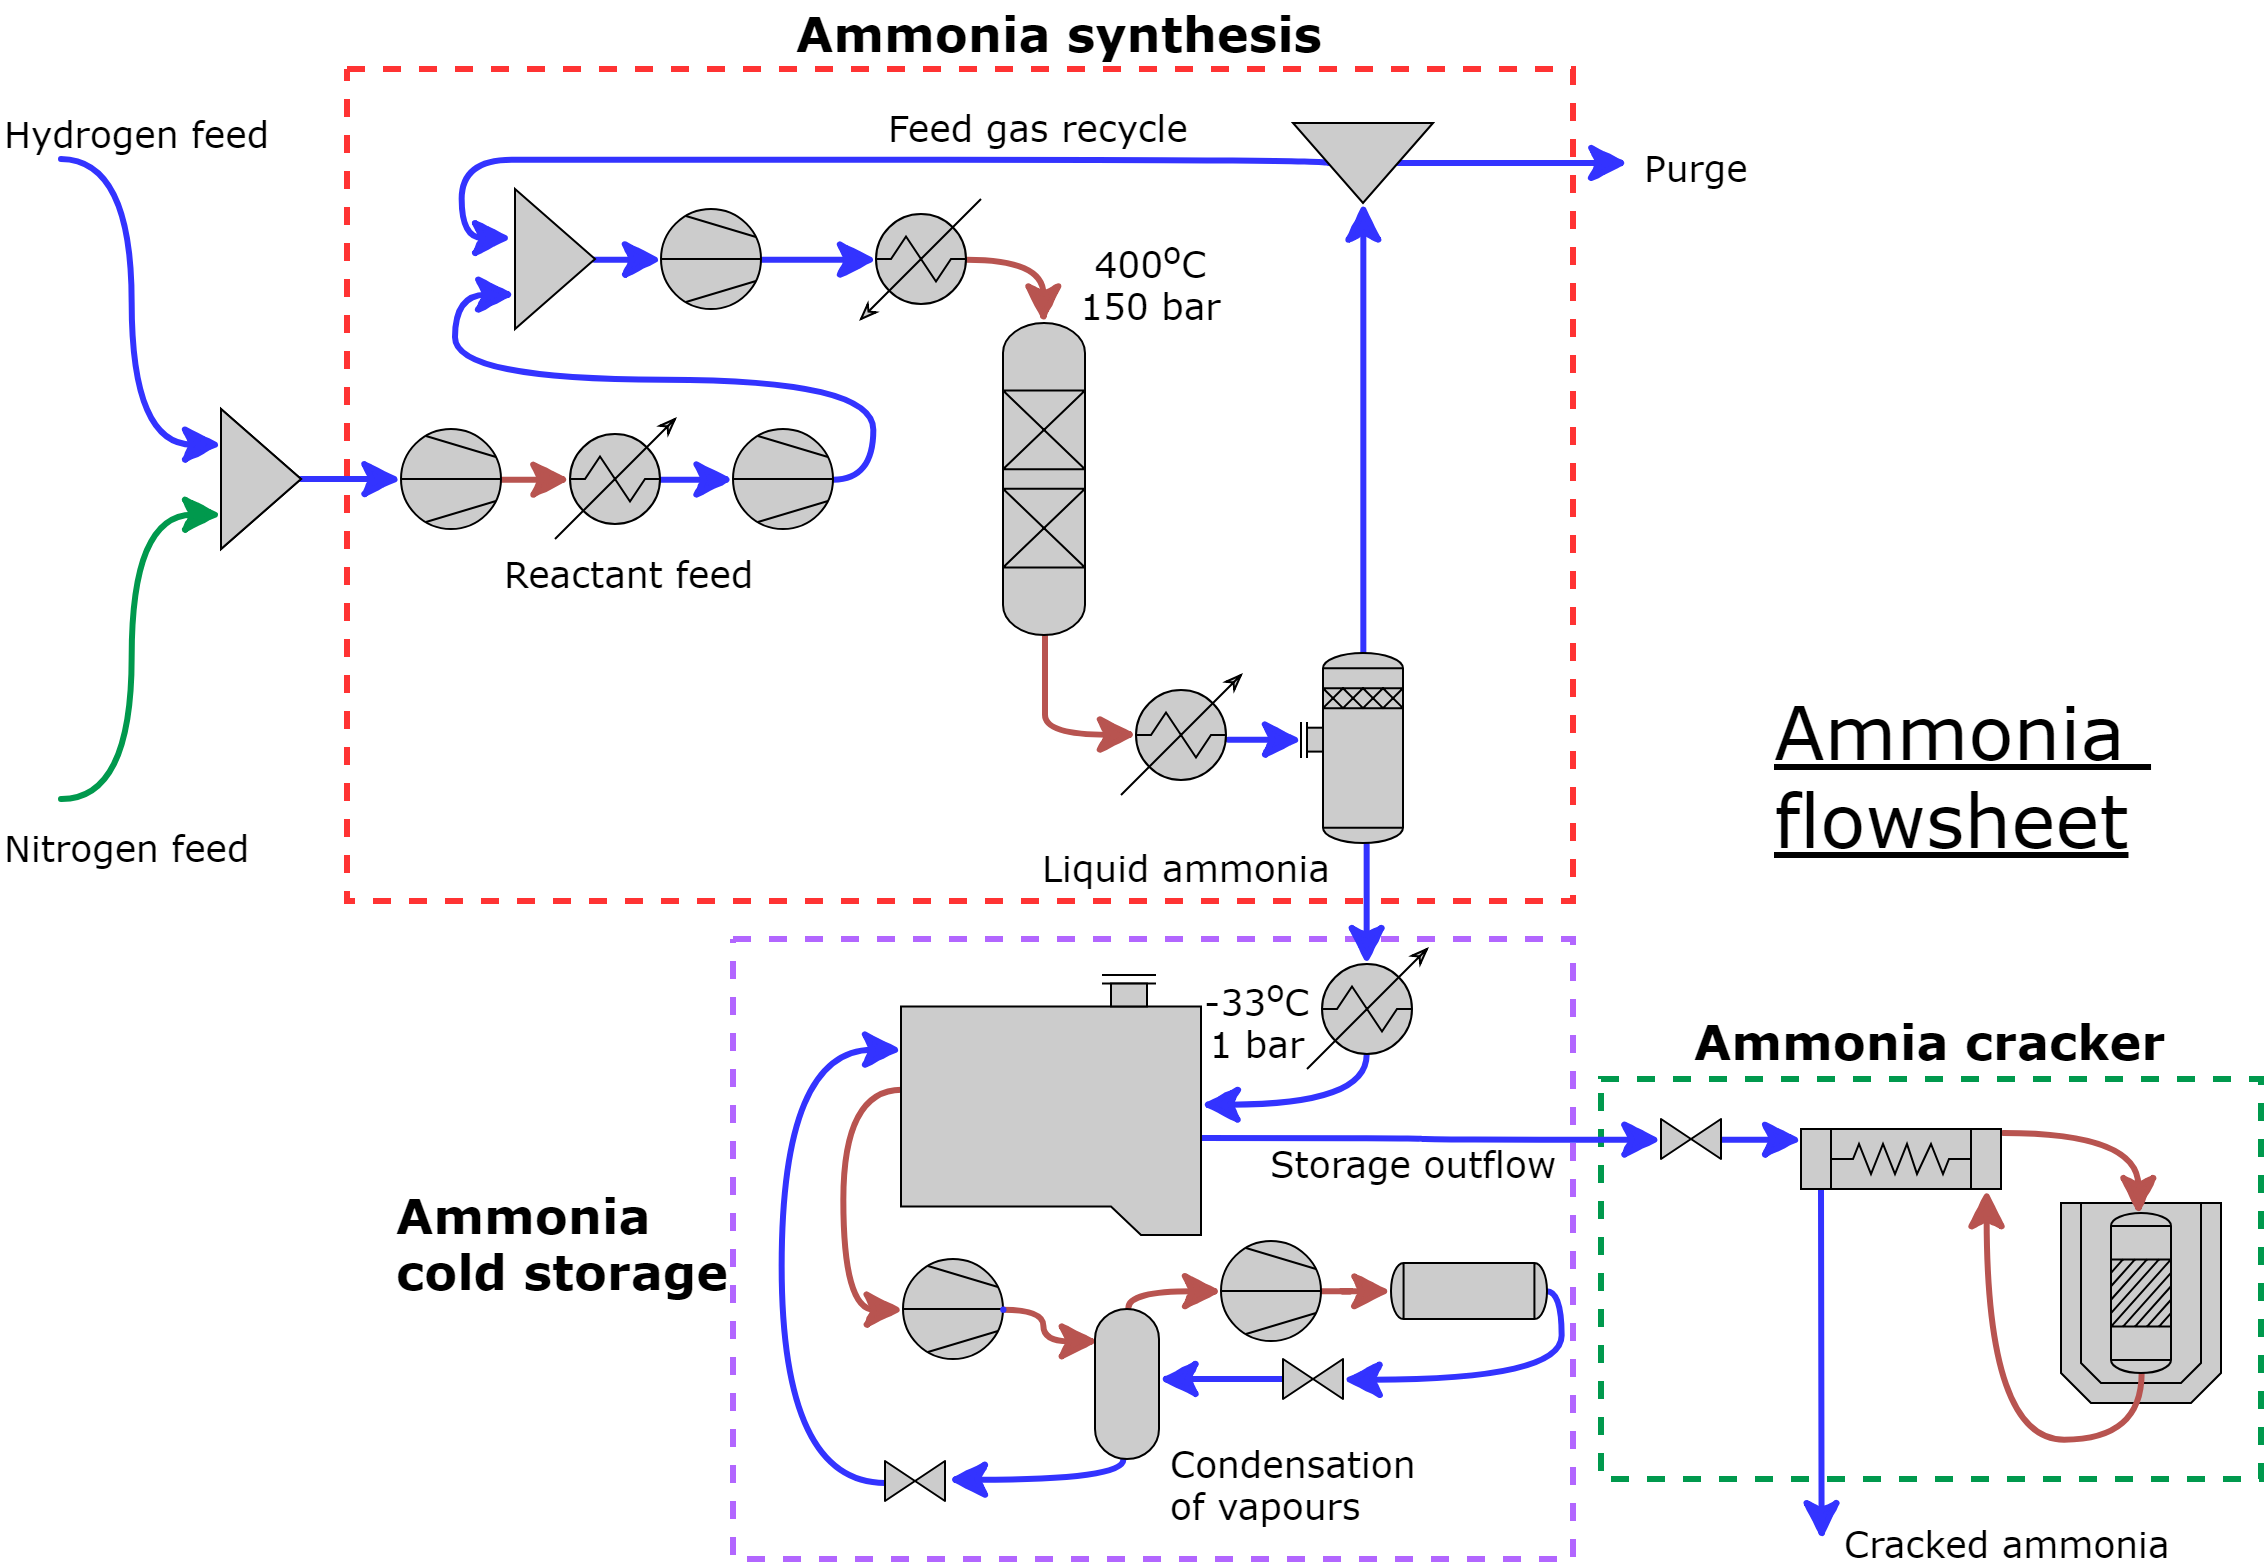
\includegraphics[width=0.95\textwidth]{ammoniasynth/handout/graphics/SSflowsheet.png}
        \caption{Ammonia Synthesis and Storage flow sheet [Slide 33]}
        \label{fig:SSflow}
    \end{figure}
   
    
    \subsection{Ammonia synthesis}
    
    
    \begin{figure}[H]
        \centering
        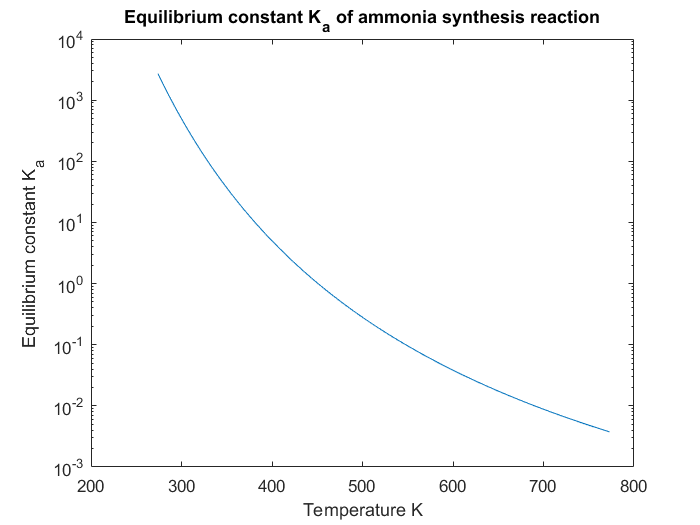
\includegraphics[width=0.60\textwidth]{ammoniasynth/handout/graphics/kc.png}
        \caption{Variation of Ka with temperature [Slide 34]}
        \label{fig:ka}
    \end{figure}
    
    {\begin{figure}[H]
		\centering
		\caption{Ammonia single pass yield as function of temperature and pressure [Slide 35]}
		{\centering
			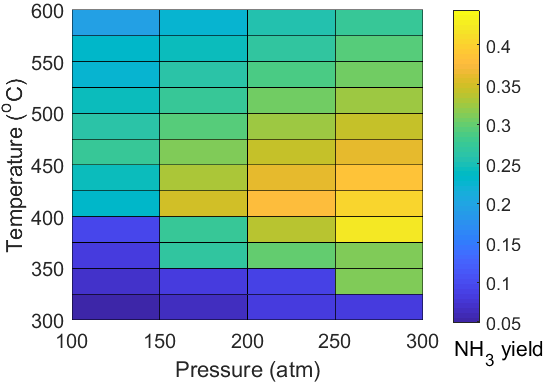
\includegraphics[width=0.46\textwidth]{ammoniasynth/handout/graphics/TPopNEW1.png}	
			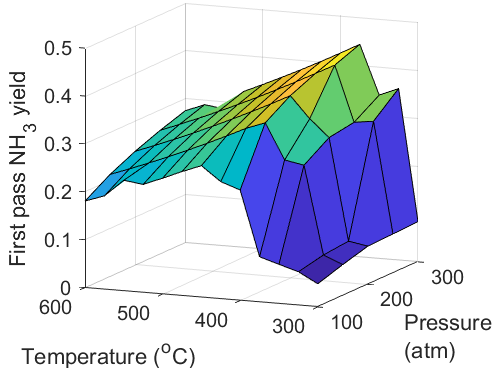
\includegraphics[width=0.46\textwidth]{ammoniasynth/handout/graphics/TPopNEW2.png}	
			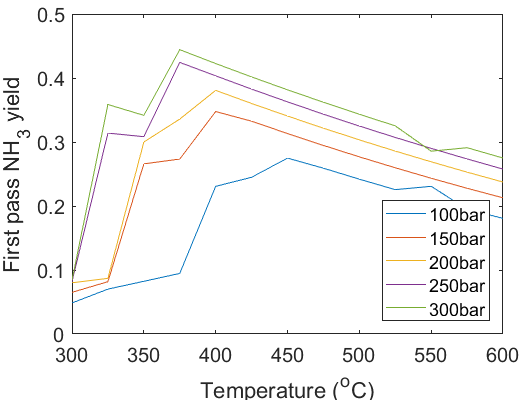
\includegraphics[width=0.6\textwidth]{ammoniasynth/handout/graphics/TPopNEW3.png}	
			 \label{fig:opt}
		}
\end{figure}}
    
    
      \begin{figure}[H]
        \centering
        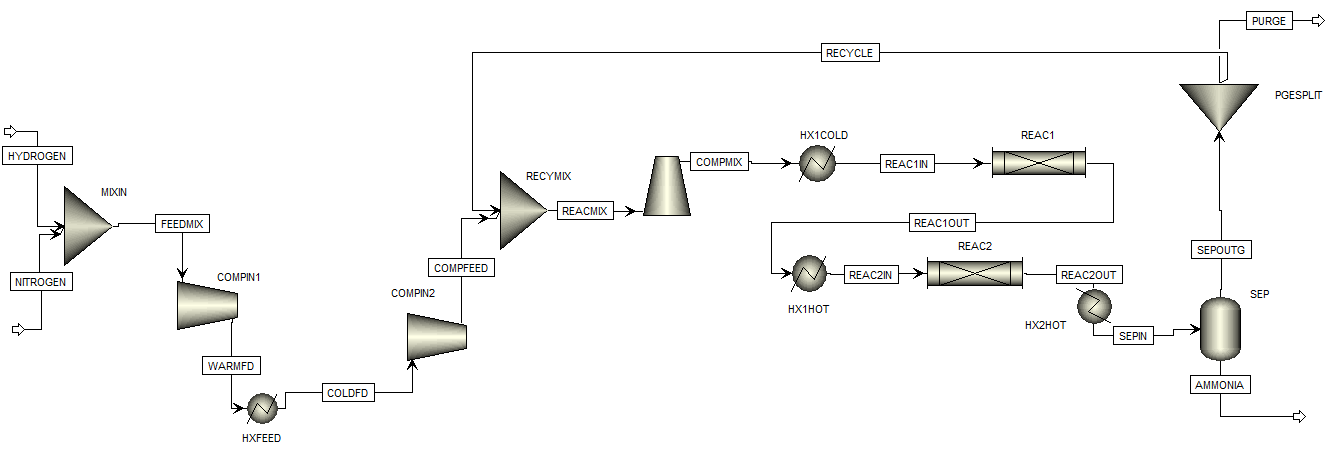
\includegraphics[width=1\textwidth]{ammoniasynth/handout/graphics/aspen}
        \caption{Aspen model of plant [Not included in presentation]}
        \label{fig:SSaspen}
    \end{figure}
    
    
        \subsection{Component design}
        
        
    \begin{figure}[H]
        \begin{subfigure}{0.5\textwidth}
            \centering
            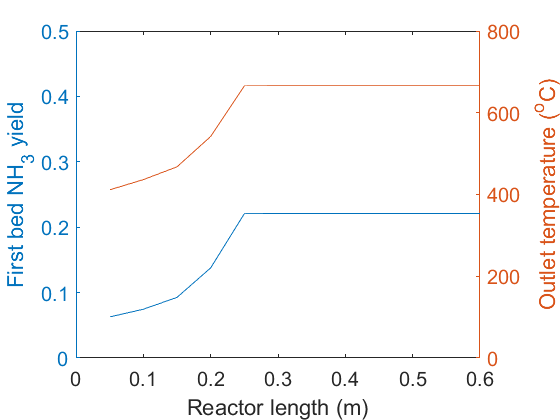
\includegraphics[width=1\textwidth]{ammoniasynth/handout/graphics/leng1.png}
            \caption{Reactor bed 1}
            \label{fig:leng1}
        \end{subfigure}%
        \begin{subfigure}{0.5\textwidth}
            \centering
            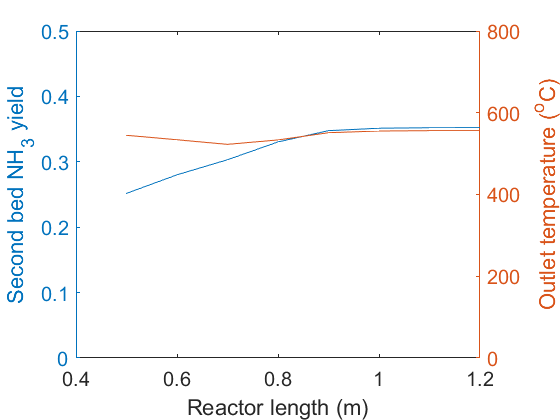
\includegraphics[width=1\textwidth]{ammoniasynth/handout/graphics/leng2.png}
            \caption{Reactor bed 2}
            \label{fig:leng2}
        \end{subfigure}
        \caption{Temperature and yield along reactor length  [Slide 36]}
    \end{figure}

        
\begin{figure}[H]

   \begin{minipage}{0.48\textwidth}
     \centering
     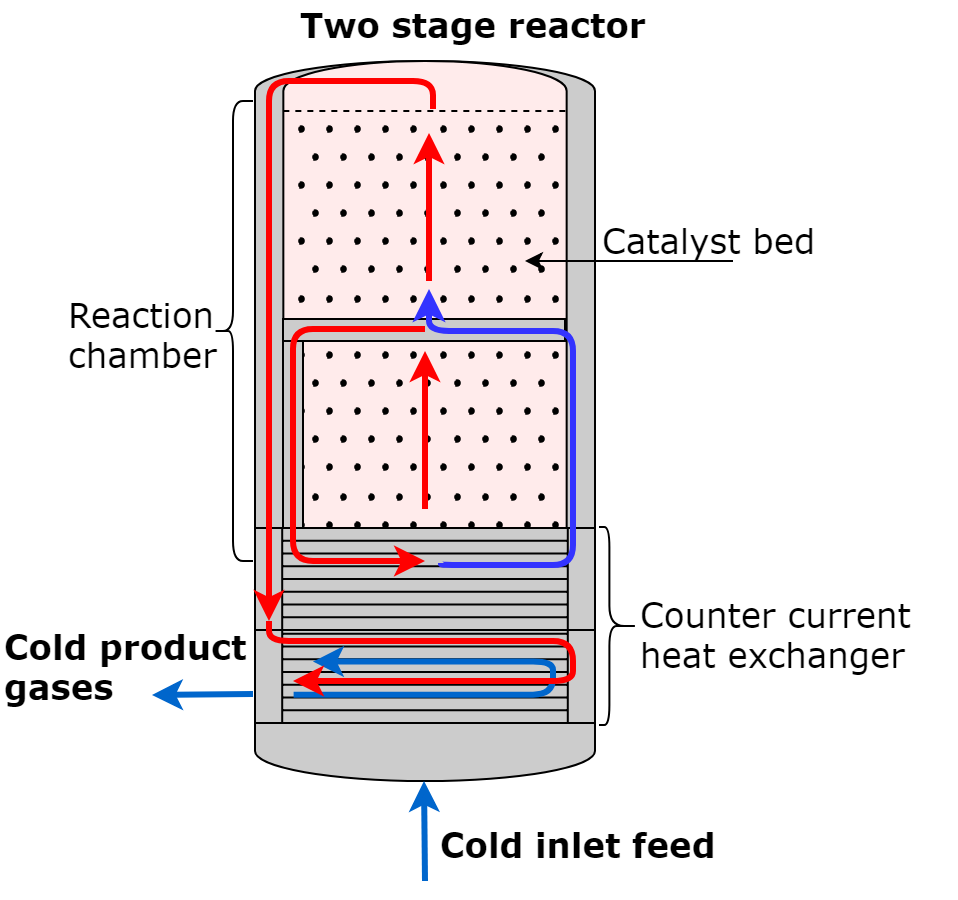
\includegraphics[width=1.05\linewidth]{ammoniasynth/handout/graphics/reac.png}
     \caption{Two bed reactor design [Slide 36]}\label{Fig:reac}
   \end{minipage}%
   \begin{minipage}{0.48\textwidth}
     \centering
     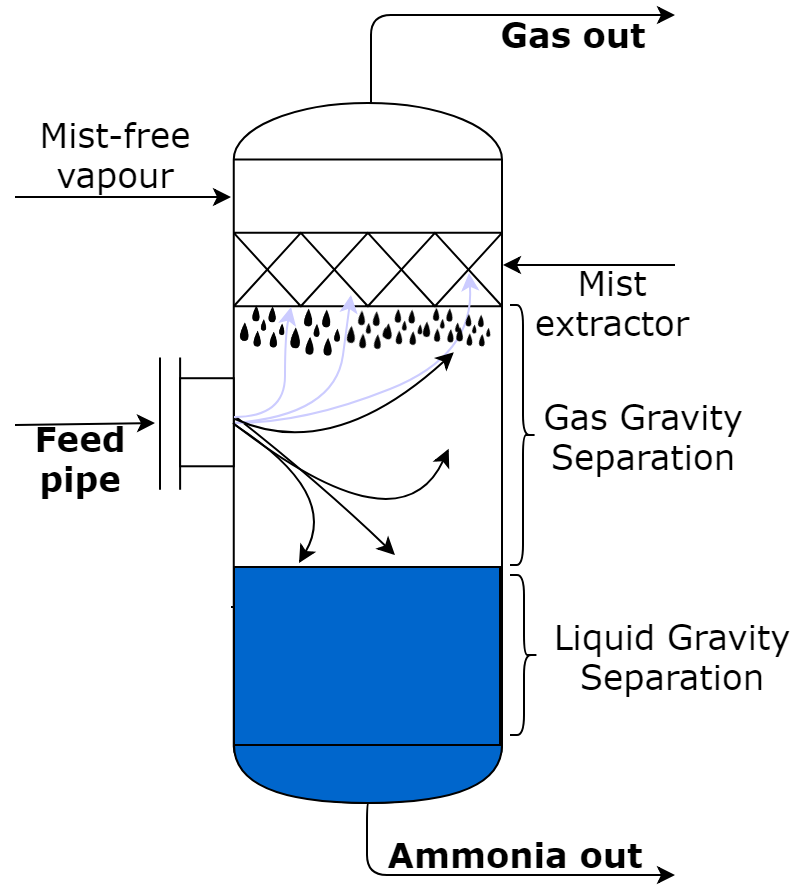
\includegraphics[width=.9\linewidth]{ammoniasynth/handout/graphics/cond.png}
     \caption{Vertical separator design [Slide 37]}\label{Fig:cond}
   \end{minipage}%
\end{figure}



            \subsection{Ammonia storage}

 \begin{figure}[H]
        \centering
        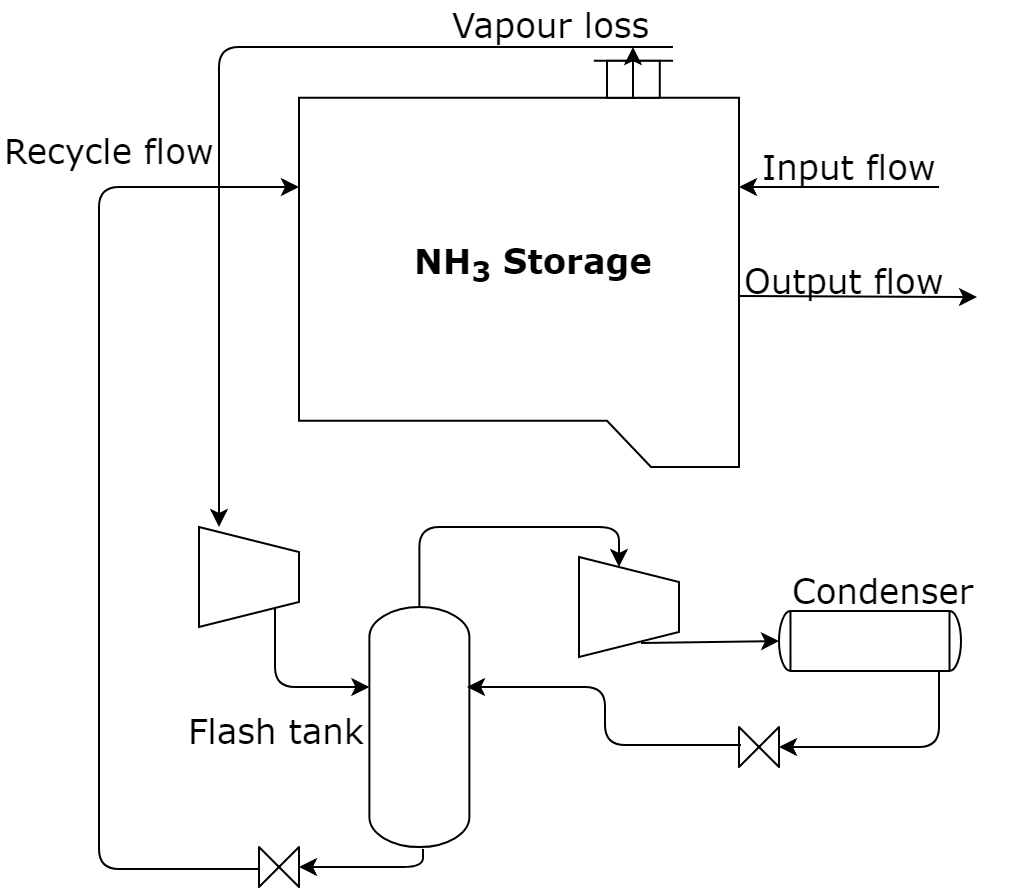
\includegraphics[width=0.5\textwidth]{ammoniasynth/handout/graphics/store.png}
        \caption{Ammonia cold storage system with recycle [Slide 38]}
        \label{fig:store}
    \end{figure}
    
    
        \subsection{Ammonia cracker}
        
 \begin{figure}[H]
        \centering
        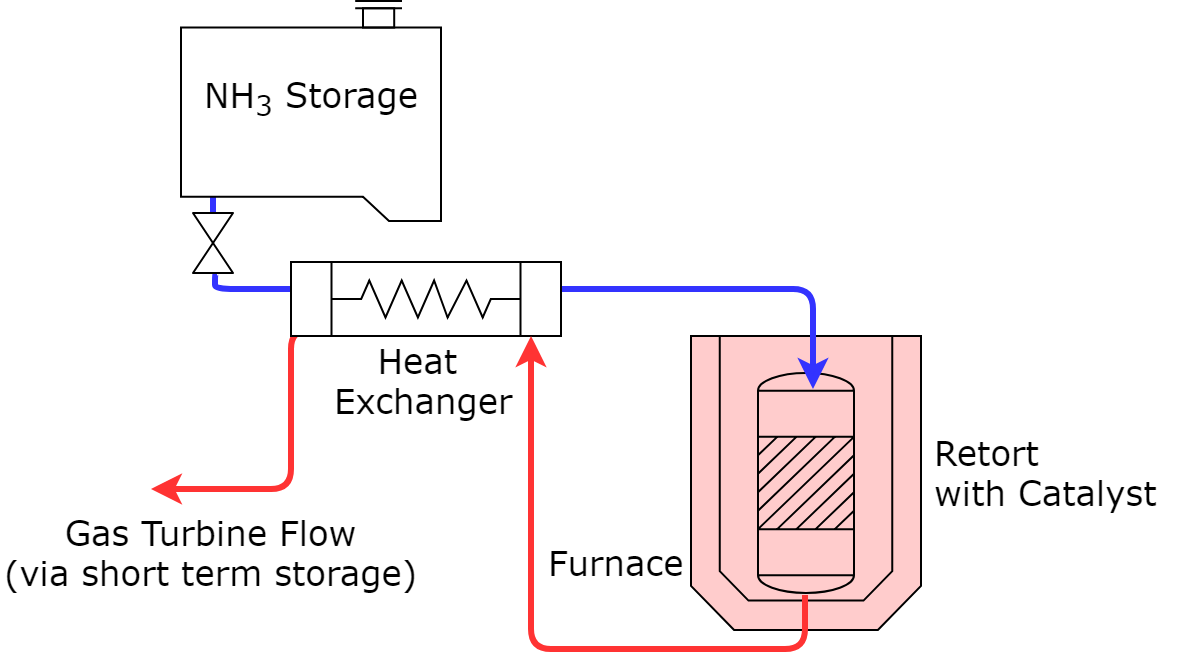
\includegraphics[width=0.65\textwidth]{ammoniasynth/handout/graphics/crack.png}
        \caption{Ammonia cracker system [Slide 39]}
        \label{fig:crack}
    \end{figure}
    
    
    \newpage
    

  %  \section{Plant Safety and Risk}

%\end{center}
%\end{document}